\newpage
\section{Desenvolvimento \label{sec:desenvolvimento}}

O programa foi desenvolvido em linguagem \texttt{C} em sistema operacional \texttt{GNU/Linux}. Além das bibliotecas convencionais \texttt{stdlib.h} e \texttt{stdio.h}, foi utilizada também a \texttt{getopt.h} para leitura de argumentos na linha comando, a \texttt{mpi.h} fornecida pelo Open MPI \cite{bib:open-mpi} e as funções e tipos de variáveis fornecidas pelo CUDA \cite{bib:cuda}.

Do MPI, usou-se apenas as principais funções como \texttt{MPI\char`_Init()},\\ 
\texttt{MPI\char`_Comm\char`_rank()}, \texttt{MPI\char`_Comm\char`_size()}, \texttt{MPI\char`_Send()}, \texttt{MPI\char`_Recv()} e \texttt{MPI\char`_Finalize()}.

Do CUDA, usou-se \texttt{\char`_\char`_global\char`_\char`_} para definir um \textit{kernel} a ser executado por cada \textit{thread} da placa de vídeo associada (\textit{device}) e as variáveis pré-definidas para definir/receber os índices das \textit{threads} e \textit{thread blocks} como \texttt{dim3}, \texttt{blockIdx}, \texttt{blockDim} e \texttt{threadIdx}.

\subsection{\textit{Smooth} -- Sequencial}

Na implementação do código sequencial, a imagem PPM P3 é lida totalmente para a memória e armazenada em uma matriz de pixels na variável \texttt{pixel\char`_t **img}. O tipo de dado \texttt{pixel\char`_t} é definido da seguinte forma: 

\texttt{typedef unsigned char pixel\char`_t[3];}

Sendo o suficiente para armazenar os valores RGB de um pixel. Foi também criada uma estrutura de dados para armazenar o cabeçalho da imagem PPM P3. Todas as estruturas de dados usadas nos programas estão definidas e documentadas no arquivo \texttt{./inc/ppm\char`_p3.h}.

Tendo lido a imagem, ela é então passada para a função \texttt{void smooth(pixel\char`_t **img, int width, int height)} que, para cada pixel da imagem, pega os valores adequados como explicado na Seção~\ref{sec:algoritmo} e ilustrado na Figura~\ref{fig:ilustracao}, e então é computada a aritmética definida na Equação~\ref{eq:aritmetica} que é atribuída ao pixel na imagem, ou seja, na variável \texttt{img}.\\

Ao final do processo, os ruídos da imagem terão sidos suavizados. Caso a imagem não contenha ruídos, o efeito \textit{smooth} acaba deixando-a mais embaçada como se percebe no exemplo da Figura~\ref{fig:lena-smooth}.

\begin{figure}[h]
	\centering
	
\includegraphics{./input/lena-smooth.png}
	\caption{Exemplo da imagem ``Lena'' \cite{bib:lena} antes e depois da aplicação do \textit{smooth}. \label{fig:lena-smooth}}
\end{figure}

\subsection{\textit{Smooth} -- Paralelo com MPI}

Para a implementação da versão paralela com MPI, usou-se as mesmas estruturas de dados da versão sequencial, inclusive a mesma função \texttt{smooth()}, porém com uma adaptação para receber uma \textit{flag} que indica o tipo de pedaço da imagem: 0 imagem inteira, 1 último pedaço, 2 primeiro pedaço e 3 pedaço intermediário. Isso foi necessário, pois ao fatiar a imagem horizontalmente, como descrito mais adiante, precisa-se enviar 2 linhas a mais para cima ou para baixo de modo que a aplicação do \textit{smooth} seja correta num pedaço na imagem.

\texttt{void smooth(pixel\char`_t **img, int width, int height, int flag)}

Como ilustrado no exemplo na Figura~\ref{fig:slice}, optou-se por fazer um fatiamento da imagem em tiras horizontais, proporcionando uma melhor divisão do trabalho qualquer que seja a quantidade de processos. Desse modo, é feito uma partição dos dados de entrada e seguido um modelo mestre-escravo, como explicado no livro-texto da disciplina \cite{bib:livro-divisao}.

Para fazer o fatiamento das regiões da imagem, seguiu-se a mesma aritmética proposta em um tutorial \cite{bib:intro} de MPI para distribuir a soma de valores de um vetor.

\begin{figure}[h]
	\centering
	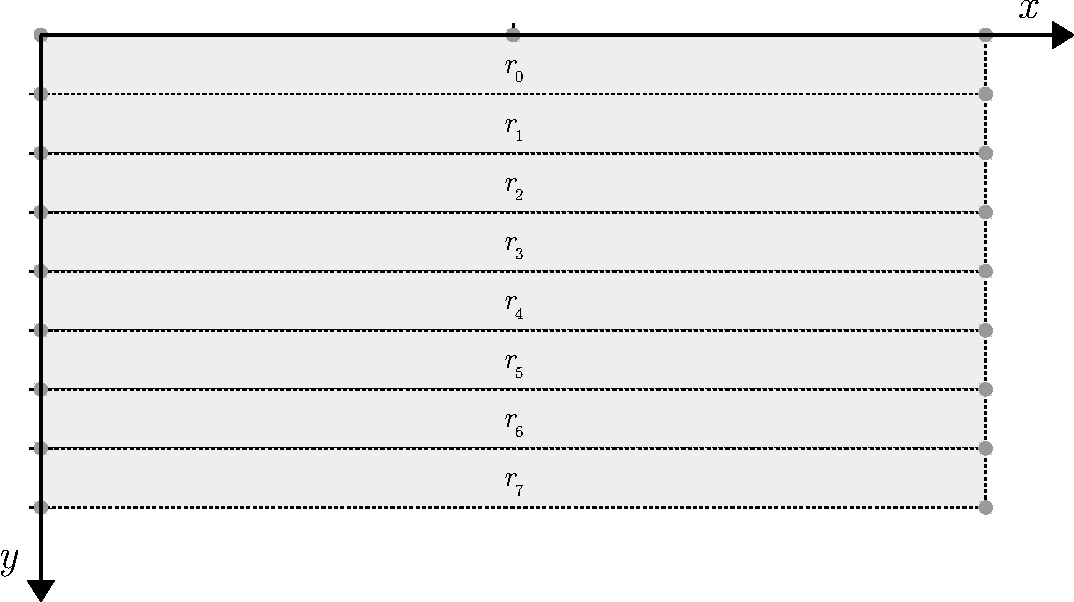
\includegraphics[scale=0.85]{./input/slice.pdf}
	\caption{Ilustração do fatiamento de uma imagem em 8 regiões. \label{fig:slice}}
\end{figure}

Considerando um exemplo de um ambiente de rede, como ilustrado na Figura~\ref{fig:hosts}, com 4 máquinas $h_i$, $i = 0, 1, 2, 3$, e criados 8 processos MPI $P_j$, $j = 0, 1, \dots, 7$ distribuídos 2 por máquina, a implementação paralela com MPI procede da seguinte forma:

\begin{enumerate}

	\item O processo \textit{master} $P_0$ localizado em $h_0$ é responsável por alocar o tamanho total da imagem em memória e ler para ela os dados que são recebidos da entrada padrão.
	
	\item $P_0$ faz o fatiamento da imagem em tiras horizontais.
	
	\item Então $P_0$ envia uma região (quantidade de linhas da imagem) para cada outro processo $P_{j \neq 0}$ localizado nas máquinas $h_i$.

\end{enumerate}


Esse exemplo é ilustrado na Figura~\ref{fig:hosts}.

\begin{figure}[h!]
	\centering
	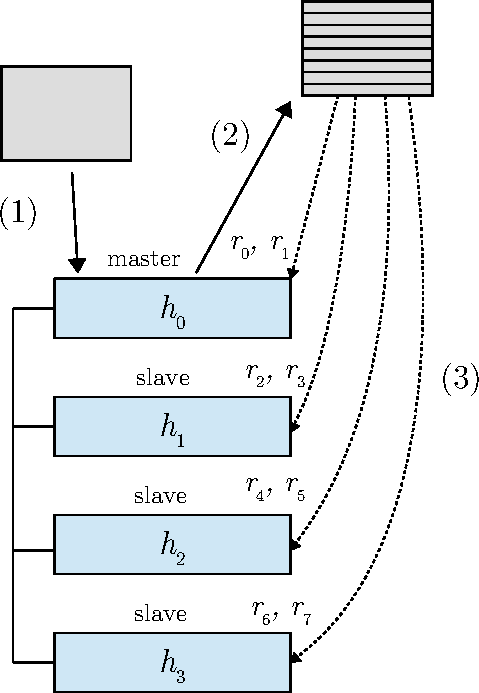
\includegraphics[scale=.85]{./input/hosts.pdf}
	\caption{Ilustração da distribuição das tarefas entres as máquinas para o exemplo. \label{fig:hosts}}
\end{figure}

Após o processamento do trabalho por cada processo MPI escravo, o resultados são enviados de volta para o processo master seguindo a ordem inversa dos fluxos da Figura~\ref{fig:hosts}. E então o processo master recompõem a imagem e retorna ela inteira com o efeito \textit{smooth} aplicado.

\subsection{Paralelo com CUDA}

Para a versão paralela com CUDA, usou-se ainda o mesmo tipo de dado \texttt{pixel\_t} para os pixels da imagem, porém, por facilidade de implementação da parte de cópia da imagem entre \textit{host} e \textit{device}, fez-se a imagem vetorizada e não mais como uma matriz.

O programa em CUDA consiste em:
\begin{itemize}
	\item Alocação de memória para a imagem no \textit{host} (\texttt{pixel\_t *img}) e no \textit{device} (\texttt{pixel\_t *img\_in, *img\_out}).
	
	\item Leitura da imagem no \textit{host} pela entrada padrão.
	
	\item Copia da imagem de \texttt{img} para \texttt{img\_in}.
	
	\item Definição da quantidade de \textit{threads} por bloco e número de blocos.
	
	\item Chamada da função \texttt{\_\_global\_\_ void cudaSmooth(pixel\_t *img\_in, pixel\_t *img\_out, int width, int height)}
	
	\item Copia do resultado de \texttt{img\_out} para \texttt{img}.
\end{itemize}

Da maneira como foi implementada, cada \textit{thread} fica responsável por calcular o \textit{smooth} de um pixel da imagem o que resulta numa execução muito rápida, pois a GPU contém uma grande quantidade de unidades lógica-aritmética. Para isso, foi usada a quantidade máxima de \textit{threads} por bloco (1024) e fazendo blocos de duas dimensões $32 \times 32$. O uso de blocos bidimensionais é de fácil associação com o problema em questão por se tratar de uma imagem que possui duas dimensões.

A função \textit{kernel} para calcular o \textit{smooth} não é a mesma usada na versão sequencial e MPI. Foi necessário criar uma nova função ligeiramente alterada para CUDA. Mais detalhes sobre sua implementação estão no código-fonte \texttt{./src/cuda.cu}.

\subsection{Cálculo das Estatísticas}

Além dos programas para a resolução do problema, foi implementado um outro programa para auxiliar o cálculo das médias, desvios padrão e intervalos de confiança dos tempos das execuções. Esse programa \texttt{./bin/stats} recebe como entrada o número de execuções seguido dos tempos de cada execução de um dos programas. O arquivo dos tempos de execução é gerado através de um \textit{shell script} \texttt{./run.sh} que roda os programas uma quantidade informada de vezes.

\subsection{Compilação e Execução dos Programas}

Estando no diretório raiz dos arquivos deste trabalho, é possível compilar e executar os programas seguindo as instruções:

\begin{itemize}
	\item Para compilar todos programas, execute: \\
		\verb|make|

	\item Para rodar a versão sequencial, execute: \\
		\verb|./bin/sequential < in.ppm > out.ppm|

	\item Para rodar a versão paralela MPI, execute: \\
		\verb|mpirun -hostfile ./hosts -np <#> -npernode <#pernode>| \\
		\verb|    ./bin/parallel < in.ppm > out.ppm|

		Por exemplo: \\
		\verb|mpirun -hostfile ./hosts -np 8 -npernode 2 ./bin/parallel < in.ppm > out.ppm|

	\item Para rodar a versão em CUDA, execute: \\
		\verb|./bin/cuda < in.ppm > out.ppm|

	\item Opcionalmente, os programas podem receber os seguinte argumentos:\\
		\verb|--no-output| ou \verb|-n| para não gerar a saída.\\
		\verb|--time| ou \verb|-t| para imprimir o tempo em segundos gasto somente com o processamento.

	\item Para limpar todos os arquivos compilados, execute: \\
		\verb|make clean|

	\item Para rodar vários testes paralelo, sequencial ou cuda, execute: \\
		\verb|./run.sh <program> <#> <#pernode> <file> <#times>|

		Exemplos: \\
		\verb|./run.sh parallel 8 2 in.ppm 10| \\
		\verb|./run.sh sequential - - in.ppm 10|\\
		\verb|./run.sh cuda - - in.ppm 10|

	\item Para conferir por vazamento de memória, execute: \\
		\verb|make memcheck|

\end{itemize}

Caso não consiga compilar e rodar os programas, confira por dependências
de uma biblioteca MPI e CUDA, assim como dos programas usados \texttt{make}, \texttt{gcc} e \texttt{valgrind}
no seu sistema operacional.

